\documentclass[12pt]{article}
\usepackage{graphicx}
\usepackage[utf8]{inputenc}
\usepackage{amsmath}
\usepackage[]{algorithm2e}
\usepackage{comment}
\usepackage{soul}
\usepackage{cancel}
\usepackage{multirow}
\usepackage{subfigure}
\graphicspath{ {images/} }
\topmargin -10mm

\headheight 10pt
\oddsidemargin 0mm
\evensidemargin -5mm
\textwidth 161mm
\textheight 210mm
\begin{document}
\thispagestyle{empty}
 \begin{center}
  A Minor Project Report\\
  \null
on\\
\null
\textbf{Prevention of Shilling attacks in Recommender systems using clustering algorithms}\\
\null

Submitted by \\
\null
\textbf{Abraham G Sebastian}\\
\textbf{13IT233}\\
\textbf{Raghav}\\
\textbf{13IT}\\
\textbf{Sagar R Alavandar}\\
\textbf{13IT233}\\
\textbf{V Sem B.Tech (IT)}\\
\null

in partial fulfillment for the award of the degree\\

of\\
\null
\textbf{BACHELOR OF TECHNOLOGY}\\
\null
In\\
\null
\textbf{INFORMATION TECHNOLOGY}\\
\null
At\\
\begin{figure}[h] % b - bottom, t - top, h - here
 \centering{
 
\includegraphics[scale=0.7]{symbol}
 }
\end{figure}
\textbf{Department of Information Technology\\
National Institute of Technology Karnataka, Surathkal.\\
July 2015}\\
\end{center}
\clearpage
\thispagestyle{empty}
\begin{center}
\underline{\textbf{CERTIFICATE}} \\
\end{center}
\null
This is to certify that the project entitled “Prevention of Shilling attacks in Recommender systems using clustering algorithms” is a bonafide work carried out as part of the course Advanced Web Technologies (IT702), under my guidance by Abraham G Sebastian, Raghav Ashok, Sagar R Alavandar, students of III Sem B.Tech(IT)  at the Department of Information Technology, National Institute of Technology Karnataka, Surathkal, during the academic semester V 2015-2016, in partial fulfillment of the requirements for the award of the degree of Bachelor of Technology in Information Technology, at NITK Surathkal.
\\
\\
\\
\\
\\
\\
\\
Place: Mangalore \hfill \line(1,0){200}

\hfill(Signature of the Guide) \\
Date: 17-08-2015\\
\clearpage
\thispagestyle{empty}
\begin{center}
\textbf{DECLARATION }\\
\end{center}
\null
I hereby declare that the project entitled “Prevention of Shilling attacks in Recommender systems using clustering algorithms” submitted as part of the partial course requirements for the course    Advanced Web Technologies (IT702) for the award of the degree of Master of Technology in Information Technology at NITK Surathkal during the Jul - Nov 2014 semester has been carried out by me. I declare that the project has not formed the basis for the award of any degree, associateship, fellowship or any other similar titles elsewhere.
Further, I declare that I will not share, re-submit or publish the code, idea, framework and/or any publication that may arise out of this work for academic or profit purposes without obtaining the prior written consent of the course Faculty Mentor and Course Instructor. 
\\ 
\\
\\
\\
\line(1,0){200}\\
(Signature of the Student)	
\\
\\
Place: Mangalore \\
Date: 17-08-2015\\
\clearpage

\section*{Abstract}


\clearpage
\tableofcontents
\clearpage
\listoffigures
\listoftables
\clearpage

\pagenumbering{arabic}
\section{Introduction}

With increase in popularity of online entertainment websites like Netflix, Amazon and Flipkart, the dependence on recommender systems is increasing.
These recommender systems are responsible for recommending items to each user based on the information available pertaining to the user.One of the more popular methods in recommender systems is collaborative filtering, which groups users with similar tastes and then chooses the items to recommend to the target user from the aggregate of preferences.   
\\
\par
	But Collaborative filtering based recommender systems are vulnerable to shilling attacks. In such attacks, the attackers generate a set of fake user profiles and give fake ratings to reduce or increase the recommendations of a certain targeted item. Shilling attacks can be divided into two types-
	  \begin{itemize}
	  	\item Push attacks - These attacks are designed to increase the popularity of a certain item so that it is recommended to more users.
	  	\item Nuke attacks - These attacks are designed to reduce popularity of a rival product so that its recommendation reduces.
	  	\\
	  \end{itemize}
\par 
    In this project, our main aim is to find the cluster of fake attack profiles. For solving this problem we assume that the fake attack profiles are a highly correlated set of users since their pattern of attack will be very similar. For finding this set of highly correlated users, we apply spectral and K-means clustering on the dataset. Since the number of items rated by each user is a small subset of the total number of items, the rating matrix (users*rating)
    is sparse. To overcome this, a similarity matrix is generated. The clustering algorithms are then applied to this similarity matrix to find the highest correlated matrix below a threshold size n.
 
\clearpage
\section{Literature Survey}
\subsection{Background }
The task allocation schemes show bad performance because of old load information. So these schemes should have some mechanism which reduces the effect of old load information. The previous approaches are based upon randomness. They focus on choosing a random node for allocating a task when old information is growing. One such strategy is Random Subset which is explained as follows:

\begin{itemize}
  \item Location strategy: Initially, a subset of nodes are selected randomly by the local node. Then the node which is having lightest load is selected. The subset of nodes is taken so that only limited number of nodes need to be searched for selecting the destination node. This is a tuning parameter in the algorithm and tries to reduce the effect of outdated load information.
  \item Information strategy: In Random Subset, each and every node dosen’t store the load related information of the all the nodes. The load information is collected on demand whenever it is required. For selecting the final destination to transfer the task, all the nodes present in the subset of local node are probed by it.
  \item Transfer strategy: Each and every time a task is arrived, the local node tries to determine on which node it should be allocated. If there is some node found on probing which has lesser load than others and that of local node, the task is transferred to that node. If it’s not found, task is executed by local node itself.
\end{itemize}


\subsection{Outcome of Literature Survey}
Our objective is to provide a task allocation scheme which is good enough to reduce effect of old load related information and performs well in context of waiting time and response time of a task. We’ll compare this approach with previously existing one and analyze the results with respect to response time, throughput etc.
\subsection{Problem Statement}
To propose a task allocation scheme that provides load balancing among the nodes and also reduces waiting time of task before being assigned to a node for processing.

\section{Proposed approach}
\subsection{Nearest Neighbor}
\paragraph{}
Nearest neighbor is distributed task allocation scheme which uses load information of nodes before allocating tasks. In Nearest neighbor approach, every node can communicate only to its neighbors. This is done in order to reduce the communication delay. This approach can be explained as follows with respect to three strategies:
\begin{enumerate}
  \item Location strategy: The destination node for transferring the task is selected among the subset of nodes called neighbors. The node with the lightest node among the neighbors is selected as destination node.
  \item Information strategy: Every node is aware of load information of its neighbors. This information is updated whenever the load of a particular node changes. It can change when some new task arrives and it is put in the queue for execution or when a task has finished executing. Receiver node updates its load related information after getting this message.
  \item Transfer strategy: Transfer strategy of nearest neighbor is same as that of Random subset. Whenever some new task is arrived, local node will try to determine appropriate destination for this. If it is not found, task will be executed by local node itself.
\end{enumerate}

\subsection{System Model and Assumptions}
Distributed system consists of many number of nodes which communicate with each other. Some communication delay is introduced due to their communication. Each node is able to process one task at a time. The task which is being executed can’t be interrupted in between. Each node is having one run queue which contains task already allocated to the node but can’t be executed immediately. The definition of load on a node is the length of its run queue. Length means number of tasks present in the queue. The size of each task is determined as the amount of calculation required for its processing.
\paragraph{}
Following assumptions are made:
\begin{itemize}

\item All tasks are independent of each other. On task’s execution makes no effect on other.
\item Node doesn’t have information about task such as burst time of task etc.
\item The communication between nodes make no effect on the execution of tasks. That means communication delay doesn’t reduce execution speed of task.

\end{itemize}

\section{Methodology}
The figure given below shows the topology used to analyze the behavior of nearest neighbor and random subset schemes. All the nodes used are of same configuration. The burst time of each task is proportional to its size and is same for each task. Neighbors of a node are the nodes which are directly connected to it.
\paragraph{}
\begin{figure}[h!]
  \centering
    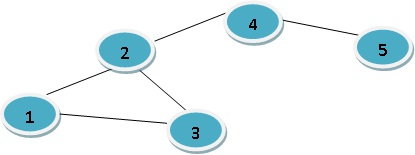
\includegraphics[width=10cm, height=6cm]{fig_1.jpg}
    \centering
    \caption{Nearest neighbor topology }
\end{figure}

\begin{itemize}
\item Arrival of tasks at the nodes is based on poisson process.
\item Each task arrived is sent to randomly selected nodes initially. Then in accordance with task allocation scheme used, they are executed locally or transferred to some other node.
\item In case of random subset scheme, The number of nodes present in subset is taken as 2.
\item The communication delay between a node and its neighboring nodes is fixed to a certain value(10ms).
\item Mean response time and waiting time are taken as performance metrics.
\par Response time = Task completion time – Arrival time
\par Waiting time = Response time – Service time
\item Simulations are performed for 1000ms.
 
\end{itemize}
\clearpage
\paragraph{Flowcharts}
\paragraph{}
The flowchart of random subset approach is shown below:
\paragraph{}
\begin{figure}[h!]
  \centering
    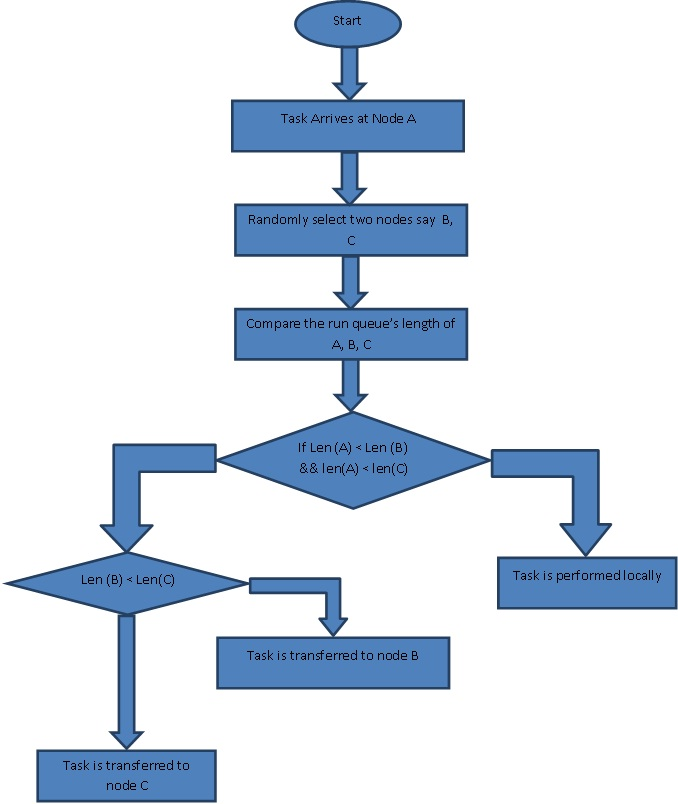
\includegraphics[width=10cm, height=16cm]{fig_2.jpg}
    \centering
    \caption{Random Subset Approach }
\end{figure}
\clearpage
\paragraph{}
The flowchart of Nearest Neighbor’s approach is shown below:
\paragraph{}
\begin{figure}[h!]
  \centering
    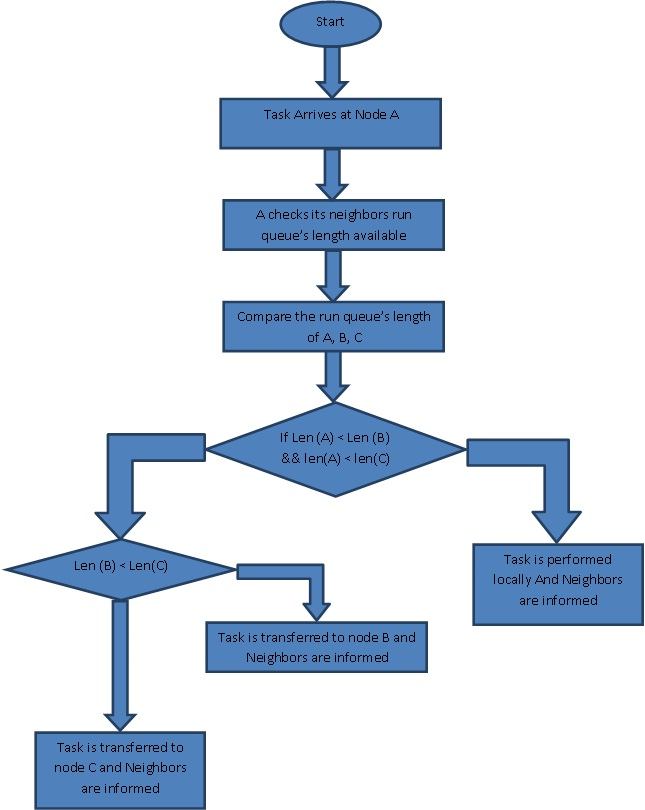
\includegraphics[width=10cm, height=16cm]{fig_3.jpg}
    \centering
    \caption{Nearest Neighbor Approach }
\end{figure}
\clearpage
\section{Implementation}
\subsection{Work Done}
Five nodes of same configuration are taken for performing simulation. At first, random subset algorithm is executed on each system parallel. It chooses two systems randomly sense them, compares the size of run queue of these systems also with the run queue of its own. Whichever system has least queue size, is selected for allocation of task. For next 1000ms, execution is continued and response time and waiting time are analyzed.
\\
\par Nearest neighbor algorithm is then executed on each system in the same way. Each node has information about its neighbors. It compares run queue length of its neighbors and along with its own run queue length. Whichever node is having least queue size, task is transferred to that node. For same period of time, this algorithm runs and response time and waiting time are compared.
\\
\\
\\
\\
\\
\subsection{Results and Analysis:}
\paragraph{Response Time}
The following table shows the values of response time noted for both the algorithms.
\paragraph{}
\begin{table}[h!]
\centering
 \begin{tabular}
{ |p{4cm}|p{4cm}|p{4cm}|  }
 \hline
 \multicolumn{3}{|c|}{Response time(in sec)} \\
 \hline
 System & Random Subset Approach & Nearest Neighbor Approach\\
 \hline
 Machine 1 & 0.17 & 0.02\\
 Machine 2 & 0.50 & 0.06\\
 Machine 3 & 0.45 & 0.05\\
 Machine 4 & 0.38 & 0.08\\
 Machine 5 & 0.28 & 0.03\\
  \hline
\end{tabular}
\paragraph{}
\centering
    \caption{Response time of Different Machines}
\end{table}
\clearpage
\paragraph{}
Above tabular values are shown in the following figure:
\\
\\
\begin{figure}[h!]
  \centering
    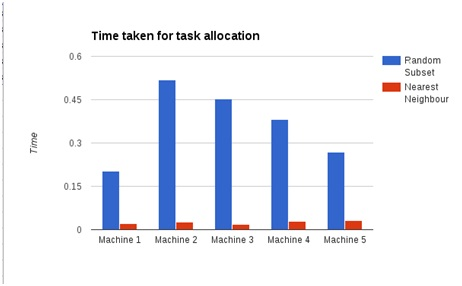
\includegraphics[width=10cm, height=7cm]{fig_4.jpg}
    \centering
    \caption{Response time graph }
\end{figure}
\\
\\
\\
\paragraph{Waiting Time}
The following table shows the values of Waiting time noted for both the algorithms.
\paragraph{}
\begin{table}[h!]
\centering
 \begin{tabular}
{ |p{4cm}|p{4cm}|p{4cm}|  }
 \hline
 \multicolumn{3}{|c|}{Waiting time(in sec)} \\
 \hline
 System & Random Subset Approach & Nearest Neighbor Approach\\
 \hline
 Machine 1 & 0.20 & 0.15\\
 Machine 2 & 0.18 & 0.16\\
 Machine 3 & 0.21 & 0.21\\
 Machine 4 & 0.11 & 0.05\\
 Machine 5 & 0.18 & 0.09\\
  \hline
\end{tabular}
\paragraph{}
\centering
    \caption{Waiting time of Different Machines}
\end{table}
\clearpage
\paragraph{}
Above tabular values are shown in the following graph:
\\
\\
\begin{figure}[h!]
  \centering
    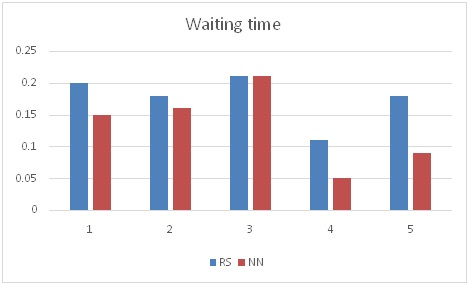
\includegraphics[width=10cm, height=12cm]{fig_5.jpg}
    \centering
    \caption{Waiting time graph }
\end{figure}

\clearpage
\section{Conclusion and Future Work}
This paper deals with task allocation schemes in large scale distributed system. In order to select the node for transferring the task, load information of task is very much useful. But the problem here is, the performance of whole system degrades if the load information is old. nearest neighbor approach is proposed in order to tackle this problem. the impact of communication delay is also reduced. It is shown that the proposed scheme gives better performance compared to the previous approach based on randomness.
\\
\par
	But the evaluation of performance is only limited to the steady-state. The task allocation scheme in general, should be able to deal with various abnormal conditions such as failure of nodes, burst arrival of tasks etc. The future work is to evaluate the proposed approach in such abnormal conditions.


\paragraph{}
 
\clearpage
\begin{thebibliography}{}
\bibitem{}
R. Mirchandaney, D. Towsley, and J. Stankovic, "Analysis of the effects of delays on load sharing," IEEE Trans. on Computers, vol. 38, no. 11, pp. 1513-1525, 1989. (Pubitemid 20642376)
\bibitem{}
M. Mitzenmacher, "How Useful Is Old Information?" IEEE Trans. On Parallel and Distributed Systems, vol. 11, no. 1, pp. 6-20, 2000. (Pubitemid 32132996)
\bibitem{}
M. Dahlin, "Interpreting stale load information," in Proc. 19th IEEE International Conference on Distributed Computing. Systems, 1999, pp. 285-296.
\bibitem{}
A. M. Alakeel, "A Guide to Dynamic Load Balancing in Distributed Computer Systems," International Journal of Computer Science and Information Security, vol. 10, no. 6, pp. 153-160, 2010.

\end{thebibliography}
\end{document}
